\section{Seconda parte - Compressione di immagini}
\subsection{Obiettivo}
    In questa seconda parte la richiesta è lo sviluppo di un piccolo \textit{sistema software} che implementi una versione semplificata della \textit{compressione} con \textit{perdità di qualità} \textbf{JPEG}, facendo utilizzo della versione fast della \textit{\textbf{DCT2}}.
    
    Anche in questo caso si è scelto di utilizzare il linguaggio \textbf{python} insieme ad un'architettura \textbf{MVC} (\textbf{Model-View-Controller}), descritta nel dettaglio nella sezione \ref{subsection:software_architecture}. 

    Inoltre, al fine di avvicinarsi il più possibile al vero formato \textbf{JPEG}, si è scelto di trattare sia immagini in \textbf{toni di grigi} che a colori (\textbf{RGB}) e di creare un proprio (banale) \textit{formato di serializzazione} (sezione \ref{subsection:jpug}); 
    
    Infine, sono stati effettuati alcuni esperimenti su immagini in formato \textbf{bmp} di varie dimensioni (sezione \ref{experiments}).

    Tutto il codice è disponibile in \href{https://github.com/iFoxz17/Jpug/tree/main/jpug}{questa repository}.

\subsection{Formato JPUG} \label{subsection:jpug}
    Come già detto, si è deciso di definire un formato personalizzato che andasse a simulare il formato \textbf{JPEG}, chiamato (in maniera fantasiosa) \textbf{JPUG}.
    Il formato salva banalmente in formato binario e in maniera sequenziale le tre componenti necessarie a ricostruire l'immagine compressa:
    \begin{itemize}
        \item il coefficiente \textbf{\textit{F}}, rappresentante la dimensione dei blocchi in cui è suddivisa l'immagine;
        \item il coefficiente \textbf{\textit{d}}, rappresentante la prima antidiagonale delle entrate da tagliare;
        \item il valore delle \textbf{entrate} (nella base dei coseni) da mantenere, che vengono linearizzate per righe in un \textbf{vettore monodimensionale}, come nel seguente esempio (per $F=5$ e $d=4$):

        $$
        \begin{bmatrix}
            a_{11} & a_{12} & a_{13} & a_{14} & - \\
            a_{21} & a_{22} & a_{23} & - & - \\
            a_{31} & a_{32} & - & - & - \\
            a_{41} & - & - & - & - \\
            - & - & - & - & - \\
            \end{bmatrix}
        \Longrightarrow 
        \begin{bmatrix}
            a_{11} & a_{12} & a_{13} & a_{14} & a_{21} & a_{22} & a_{23} & a_{31} & a_{32} & a_{41}
        \end{bmatrix}
        $$
    \end{itemize}
    Il \textbf{numero \textit{n} di entrate} della matrice \textbf{da mantenere} (\textbf{dimensione del vettore linearizzato}) sarà dato da:
    \begin{itemize}
        \item Per $ 0 \le d \le F$:
        \begin{equation}
        n = \sum_{i=0}^{d-1}{i+1} = \sum_{i=1}^{d}{i} = \frac{d(d+1)}{2}
        \end{equation}
        
        \item Per $ F < d \le 2F - 1$:
        \begin{equation}
        n = \frac{F(F+1)}{2} + \sum_{k=1}^{d-F}{F-k}
        \end{equation}
        dove
        \begin{align*}
            \sum_{k=1}^{d-F}{F-k} &= \sum_{k=1}^{d-F}{F} - \sum_{k=1}^{d-F}{k} = \\
                             &= F(d - F) - \frac{(d - F)(d - F + 1)}{2} = \\
                             &= Fd - F^2 - \frac{1}{2}d^2 + \frac{1}{2}Fd - \frac{1}{2}d + \frac{1}{2}Fd - \frac{1}{2}F^2 + \frac{1}{2}F = \\
                             &= -\frac{3}{2}F^2 + \frac{1}{2}F + 2Fd - \frac{1}{2}d^2 - \frac{1}{2}d
        \end{align*}
        e di conseguenza
        \begin{align*}
        n &= \frac{1}{2}F^2 + \frac{1}{2}F - \frac{3}{2}F^2 + \frac{1}{2}F + 2Fd - \frac{1}{2}d^2 - \frac{1}{2}d = \\
          &= 2Fd - \frac{1}{2}d^2 - F^2 - \frac{1}{2}d + F
        \end{align*}
    \end{itemize}
    Riassumendo:
    \begin{equation}
    n(F, d) = \begin{cases}
              \frac{d(d+1)}{2} & \text{se } 0 \le d \le F \\
              2Fd - \frac{1}{2}d^2 - F^2 - \frac{1}{2}d + F & \text{se } F < d \le 2F - 1
            \end{cases}
    \end{equation}
    La \textbf{percentuale di entrate salvate} (o \textbf{tasso di compressione}) $\delta$ sarà invece dato da:
    \begin{equation}
        \delta(F, d) = \frac{F^2 - n}{F^2} = 1 - \frac{n}{F^2}
    \end{equation}
    che vale
    \begin{itemize}
        \item $0 \le d \le F$:
        \begin{equation}
            \delta(F, d) = 1 - \frac{d(d+1)}{2F^2}
        \end{equation}
        
        \item $ F < d \le 2F - 1$:
        \begin{equation}
            \delta(F, d) = 1 - \frac{4Fd - d^2 - 2F^2 - d + 2F}{2F^2} = 2 - \frac{4Fd - d^2 - d + 2F}{2F^2}
        \end{equation}
    \end{itemize}

    \begin{figure}[h]
        \centering
        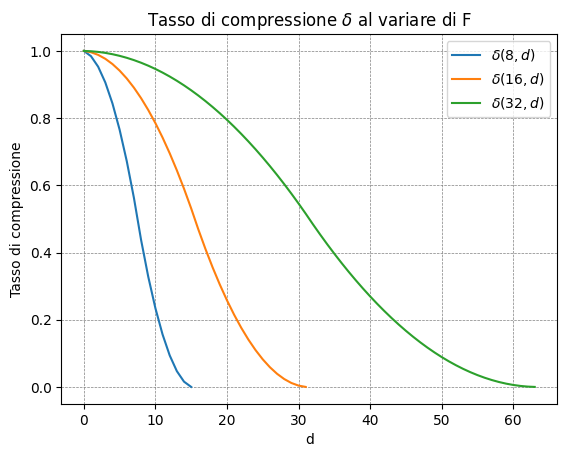
\includegraphics[width=0.5\textwidth]{images/compressione_rate_plot.png}
        \caption{\textbf{Tasso di compressione} $\delta$ per diversi valori di $F$}
        \label{fig:compression_rate_plot}
    \end{figure}
    Si noti che sia $n$ sia $\delta$ fanno riferimento al \textit{numero di elementi} dei blocchi ma \textbf{non direttamente} alla \textit{quantità di spazio effettivo (in byte)}: infatti, data l'assenza di utilizzo di una \textbf{matrice di quantizzazione}, questo formato 'naive' salva gli elementi dei vettori compressi come \textbf{numeri a virgola mobile}, che quindi occupano \textbf{2, 4} o \textbf{8 bytes} (a seconda della precisione richiesta), a differenza dei singoli \textbf{byte} delle immagini originali. Questo comporta che, per valori di $d$ non abbastanza piccoli, l'effetto sia quello di \textbf{aumentare la dimensione dell'immagine} anzichè diminuirla (nonostante ci sia comunque perdita di qualità).

    Nel caso di immagini \textbf{RGB}, vengono compresse e salvate tutte e tre le matrici \textbf{R}, \textbf{G} e \textbf{B} in maniera indipendente.
    
\subsection{Architettura di sistema} \label{subsection:software_architecture}

    \begin{figure}[ht]
        \centering
        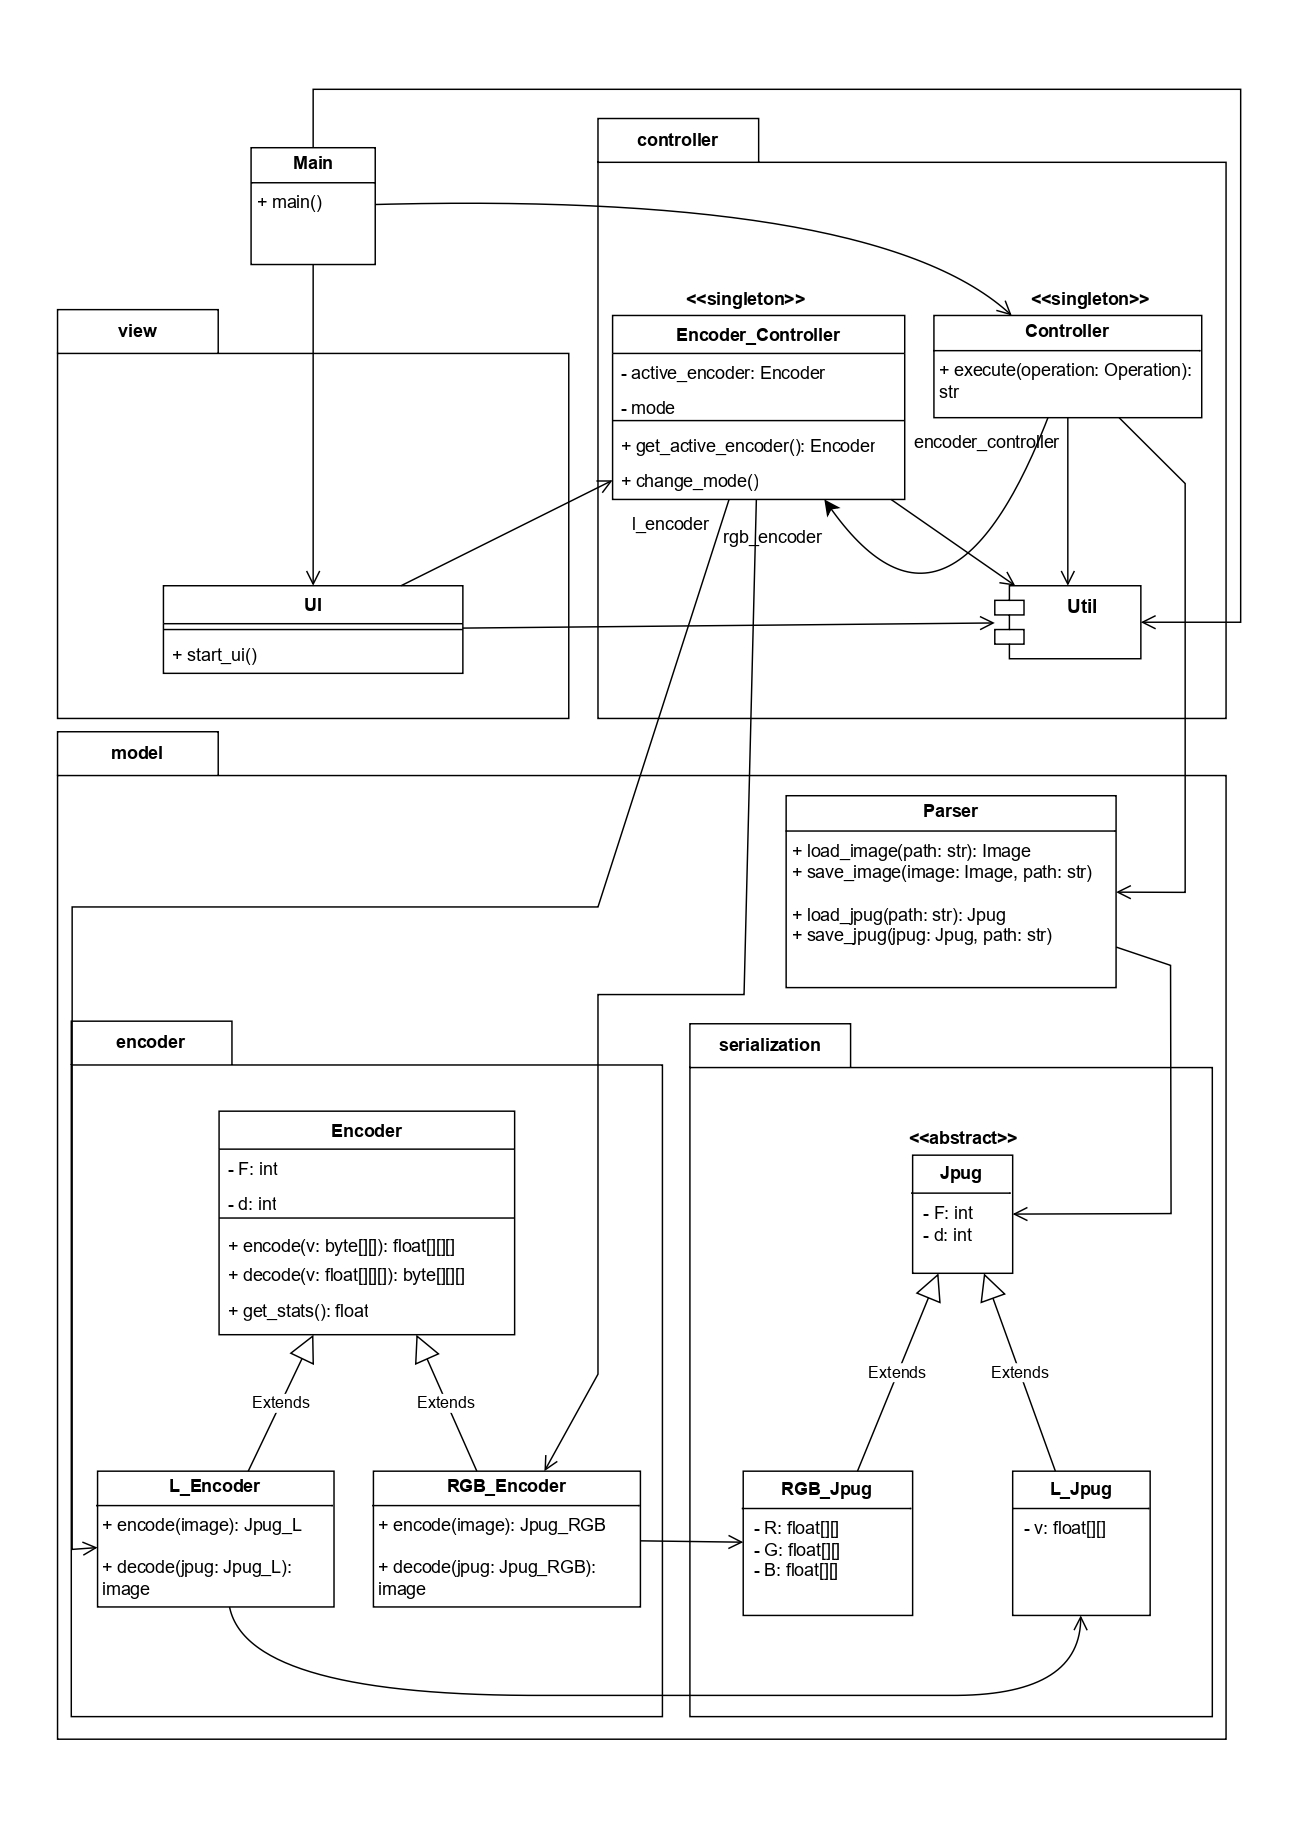
\includegraphics[width=0.8\textwidth]{images/class_diagram.jpg}
        \caption{Diagramma delle classi}
        \label{fig:class_diagram}
    \end{figure}

\subsection{Esperimenti} \label{experiments}